\chapter{Marco Te\'orico}
\label{cap:marcoTeorico}

\section{Streaming}
\label{sec:streaming}

Streaming es una t\'ecnica para la transferencia de datos de forma continua, de tal manera que sea temporal y secuencial, cuyo funcionamiento se basa en el env\'io de datos por parte de un ente externo a un sistema de procesamiento de informaci\'on. \normalsize{En caso} de estar ocupado el servicio, se dejan los datos en cola \citep{Menin2002SMH}. Generalmente, esto es utilizado en la interacci\'on con la Web, como redes sociales o reproducci\'on \textit{online} de contenido multimedia. En la Figura \ref{fig:streaming} se muestra un servidor \normalsize{del} que emana un flujo de datos que llega a distintos clientes, donde cada uno de ellos procesa la informaci\'on entrante, y en caso de estar ocupado el sistema, se guarda en un \textit{buffer} los datos para posteriormente ser procesados.

\begin{figure}[ht!]
  \centering
    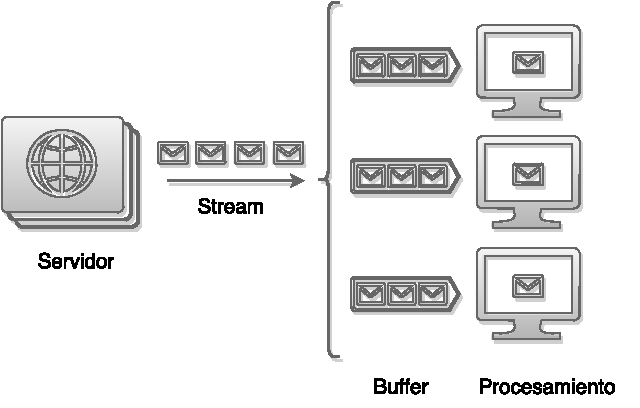
\includegraphics[scale=0.7]{images/Streaming.pdf}
  \caption{Flujo de datos entre el servidor y los clientes.}
  \label{fig:streaming}
\end{figure}

Este tipo de t\'ecnica es \'util cuando se desea procesar informaci\'on en tiempo real, siendo relevante la temporalidad de los datos, como la reproducci\'on \textit{online} de material multimedia. Los datos emanados por el \textit{streaming} pueden ser utilizados para el an\'alisis y procesamiento de un SPS (Sistema de Procesamiento de \textit{Stream}). Un ejemplo de esto es la \textit{Streaming API} proporcionada por Twitter, donde esta informaci\'on se puede utilizar para estudiar los \textit{tweets}, los \textit{trending topic} o los \textit{hashtag} m\'as utilizados para casos espec\'ificos como campa\~nas electorales o desastres naturales.

\section{Stream processing}
\label{sec:streamProcessing}

\textit{Stream processing} es un paradigma de programaci\'on, orientado al procesamiento de un flujo de datos en tiempo real. Se centra en la programaci\'on de aplicaciones que puedan procesar la informaci\'on en el momento, utilizando los recursos del sistema de forma paralela o distribuida para cumplir su objetivo, de tal manera que su procesamiento sea lo m\'as cercano al tiempo real \citep{ChakravarthyJ09}.

Dentro de las aplicaciones existentes en el procesamiento de \textit{stream}, est\'an el monitoreo de signos vitales, detecci\'on de fraudes, reproducci\'on de videos \textit{online}. Para el funcionamiento correcto de estas aplicaciones, es necesario cumplir con ciertas caracter\'isticas. \citep{andrade2014fundamentals} establece los requerimientos para el procesamiento continuo de datos, estos se desglosan a continuaci\'on::

\begin{itemize}
	\item \textbf{Procesamiento de grandes cantidades de datos}: esto significa que al tratar de procesar los datos, no se puede guardar en una base de datos y luego procesarlos, como en general lo realizan los sistemas de \textit{bash processing}. Por lo tanto es necesario otro mecanismo que pueda procesarlos mientras va llegando la informaci\'on entrante. \normalsize{\textit{Stream processing}} soluciona este problema, dado que la informaci\'on entrante es procesada a medida que van llegando los datos.
	\item \textbf{Limitaciones de ancho de banda y latencia}: se refiere a la comunicaci\'on que existe por parte del proveedor de datos, de tal manera que no sea una limitante en el procesamiento de los datos el ancho de banda o la latencia existente. Esto es importante, dado que no sirve un sistema de estimaci\'on de la bolsa del mercado si es que presenta alta latencia. Siempre se debe mantener una baja latencia, para poseer los datos lo m\'as cercano al tiempo real.
	\item \textbf{Procesamiento de datos heterog\'eneos}: en su mayor\'ia, los datos poseen distintos formatos, contenidos y niveles de ruido, por lo que es necesario realizar una normalizaci\'on de estos, de tal manera de estandarizar el procesamiento.
	\item \textbf{Proporcionar alta disponibilidad a largo plazo}: es importante poseer un constante flujo de informaci\'on, que sea estable y persistente en el tiempo, de tal manera que est\'e procesando constantemente los datos para el prop\'osito designado. Si analizamos el funcionamiento de los sistemas, estos poseen un porcentaje de fallas, y los SPS no son la excepci\'on, por ello es importante contar con un mecanismo de tolerancia a fallos que permita reducir la p\'erdida de informaci\'on. De no existir, se puede perder informaci\'on, comprometiendo la precisi\'on de los resultados y requiriendo de un mayor tiempo para recolectar la informaci\'on perdida o alcanzar un estado similar.
\end{itemize}

\section{Sistemas de procesamiento de stream}
\label{sec:SPS}

Entre los diferentes motores de procesamiento de datos masivos, existen los sistemas de procesamiento de \textsl{stream}, los cuales reciben grandes cantidades de datos que deben procesar de forma distribuida y en tiempo real, de ahora en adelante hablaremos de procesamiento \textsl{online} para hacer referencia al tiempo real. Para realizar esto, se requiere un cambio en el paradigma tradicional de \textsl{bash processing}, el cual almacena los datos, para posteriormente procesarlos de manera \textit{offline} \citep{HawwashN14}. Este cambio de paradigma implica el an\'alisis de datos sin requerir su almacenamiento, de esta manera los datos fluyen mientras son procesados.

El paradigma utilizado se basa en grafos de procesamiento como muestra la Figura \ref{fig:grafo}, donde los operadores (o tareas de procesamiento) corresponden a las v\'ertices del grafo, como por ejemplo analizadores de sentimientos, filtros de palabras o alg\'un algoritmo en particular, y las aristas corresponden a los flujos de datos entre un operador y otro \citep{Shahrivari14}. Adem\'as de esto, los datos proporcionados son originados por un ente externo, ya sea \textit{streaming} de redes sociales, estad\'isticas del monitoreo de un sistema, o transacciones en la bolsa de comercio, la cual entrega los datos iniciales a los primeros operadores del grafo \citep{AppelFFB12}.

\begin{figure}[ht!]
  \centering
    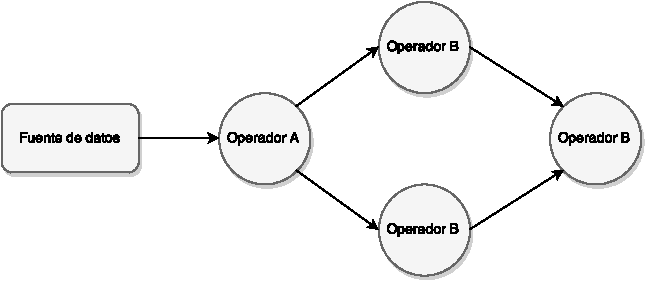
\includegraphics[scale=1]{images/SPS.pdf}
  \caption{Ejemplo de modelo de SPS.}
  \label{fig:grafo}
\end{figure}

Cabe destacar que los SPS son distribuidos, es decir, cada uno de los v\'ertices del grafo son alojados en un nodo f\'isico disponible en el ambiente en que se aloja el sistema, ya sea un \textit{cluster}, un \textit{grid} o un \textit{cloud}. Para lograr la comunicaci\'on entre los operadores, se utilizan sistemas anexos especialmente dise\~nados para este tipo de tareas, como Apache ZooKeeper \citep{HuntKJR10}. Este \'ultimo consiste en un servicio centralizado que mantiene informaci\'on de configuraci\'on y sincronizaci\'on de las aplicaciones distribuidas que se posean. \normalsize{Para esto, cada nodo de procesamiento debe registrarse en el sistema, y es el servidor central el que posteriormente se encarga de se\~nalar los nodos disponibles para el procesamiento y distribuir los eventos entre ellos.}

Las principales aplicaciones que se le dan a estos SPS, est\'an orientadas al manejo de grandes cantidades de datos, las cuales deben ser procesadas para obtener informaci\'on o estad\'isticas, como es el caso de detecci\'on de fraudes, recolecci\'on de informaci\'on en caso de desastres o an\'alisis de la interacci\'on en las redes sociales. Para efectuar un procesamiento en tiempo real de los datos, \citep{StonebrakerCZ05} establece los siguientes requerimientos:

\begin{itemize}
	\item \textbf{Baja latencia}: este concepto est\'a asociado con la comunicaci\'on fluida entre los distintos nodos del sistema, de tal manera que no existan altos \textit{delay} o retrasos en el procesamiento.
	\item \textbf{Consultas SQL}: poder realizar consultas a una base de datos, sin perder las propiedades del SPS, como el procesamiento distribuido. Para esto, se debe realizar un cambio en la forma de ejecutar las consultas, debido que no s\'olo es necesario realizar la consulta, sino tambi\'en que se pueda unir las respuestas entregadas de forma paralela. Dado lo anterior, se hace necesario dise\~nar un sistema que cumpla con operadores adicionales a los utilizados en las consultas tradicionales por sistemas centralizados.
	%\item \textbf{Manejo de fallas en el flujo de dato}: es importante poseer sistemas que no se preocupen de la p\'erdida en los datos, debido que se posee como premisa que se van a perder datos en el procesamiento de estos, ya sea por las colas, \textit{delays} u otro problema asociado al procesamiento o la fuente de datos. Por lo tanto, al modelar la aplicaci\'on no es necesario lidiar con este tipo de fallas.
	\item \textbf{Generar resultados predecibles}: cuando se realizan consultas en el sistema, existe la posibilidad que sean correctas s\'olo por un per\'iodo de tiempo, debido a alguna falla en el sistema que genere una p\'erdida en el estado del operador. Por lo tanto, es necesario garantizar que el resultado sea determin\'istico y persistente en el tiempo, ya sea respaldando la informaci\'on u otro mecanismo, de tal manera que si se realiza una consulta, el resultado sea consistente u hom\'ologo con el transcurso del tiempo.
	\item \textbf{Integrar almacenamiento y flujo de datos}: en general, cuando se trabaja con procesamiento de datos, es importante guardar estados en el sistema, de tal manera que los datos entrantes vayan verificando, modificando o eliminado la informaci\'on que se posea. En un operador que cuente palabras, es necesario soportar variables que guarden las estad\'isticas de la informaci\'on entrante. Otro tema importante es la uniformidad de los datos, como se hab\'ia explicado anteriormente, en general se trabaja con datos heterog\'eneos, por lo que se requiere estandarizarlos para su procesamiento, de tal manera que no exista una discordancia en la informaci\'on procesada.
	\item \textbf{Garantizar la seguridad y disponibilidad de los datos}: este requerimiento est\'a orientado \normalsize{a disponer de} mecanismos de \textit{checkpoint}, t\'ecnica utilizada para respaldar el estado del operador cada cierto per\'iodo de tiempos. Por lo que en caso de existir alguna falla, el sistema pueda volver a estar disponible sin perder una cantidad considerable de informaci\'on, ya sea en las estad\'isticas o estados del sistema.
	\item \textbf{Partici\'on y escalabilidad autom\'atica de las aplicaciones}: es importante tambi\'en distribuir la carga entre los distintos procesadores o m\'aquinas, deseando idealmente una escalabilidad incremental. Esto significa que el flujo de datos sea entregado a los distintos recursos que se poseen, y en caso de necesitar m\'as recursos incrementarlos \citep{bookTanenbaum}. Si bien no sucede siempre, se espera que esto sea autom\'atico y transparente.
	\item \textbf{Procesamiento y respuesta instant\'anea}: cuando se plantea el uso de los SPS, se apuesta por un sistema que entregue respuestas en un tiempo lo m\'as cercano al real. Este requerimiento hace necesario lidiar posibles sobrecargas de los operadores, las cuales afectan al rendimiento del sistema. Por lo tanto, se hace necesario abordar estos posibles escenarios proveyendo una soluci\'on de bajo \textit{overhead}, \normalsize{es decir} con bajo costo de implementaci\'on o recursos necesarios para su funcionamiento, aumentando as\'i la eficiencia y el rendimiento del sistema.
\end{itemize}

Cada sistema de procesamiento de \textsl{streaming} est\'a basado en un modelo de procesamiento en particular. Por ejemplo, S4 utiliza el modelo de procesamiento \textsl{push} \citep{s4yahoo}, y Storm el modelo \textsl{pull} \citep{stormtwitter}.

El primer modelo llamado \textit{push} consiste en el env\'io de datos desde el operador \normalsize{al pr\'oximo operador seg\'un la topolog\'ia del grafo}. La ventaja de este modelo empleado por S4 radica en la abstracci\'on en el env\'io de datos, sin embargo no asegura el procesamiento de estos, debido a que no existe un mensaje de respuesta al ser entregado al operador. En la Figura \ref{fig:sps-push} el Operador A env\'ia los datos al Operador B, donde en caso que el Operador B est\'e procesando un dato, \'este lo guarda en cola. \normalsize{Dada la forma en como se realiza el env\'io, \'este no asegura que llegue el dato, debido a que no existe una respuesta por parte del operador receptor. Por lo tanto, existe una abstracci\'on en el env\'io de los eventos por parte del operador receptor, debido que no es necesario saber de qui\'en es el operador receptor.}

\begin{figure}[ht!]
  \centering
    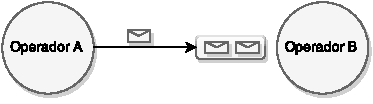
\includegraphics[scale=1]{images/SPS-Push.pdf}
  \caption{Modelo push de procesamiento.}
  \label{fig:sps-push}
\end{figure}

Por otra parte, el segundo modelo llamado \textit{pull}, se basa en la petici\'on de datos a un operador, por lo que son enviados solo s\'i son requeridos. Si bien este modelo asegura procesamiento de los datos, genera una menor abstracci\'on al programador, dado que en el primer modelo s\'olo se indica a \normalsize{qu\'e} operador deben ir los datos, en cambio en el segundo se debe indicar qui\'en lo env\'ia y qui\'en lo recibe. En la Figura \ref{fig:sps-pull} (a) se observa que existen dos operadores, donde se solicita por parte del Operador B el env\'io de un dato para ser procesado, para que posteriormente en la Figura \ref{fig:sps-pull} (b) el Operador A env\'ia el dato para que posteriormente sea procesado por el Operador B.

\begin{figure}[ht!]
  \centering
    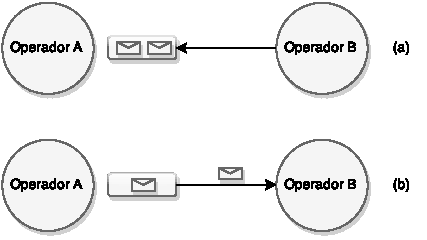
\includegraphics[scale=1]{images/SPS-Pull.pdf}
  \caption{Modelo pull de procesamiento.}
  \label{fig:sps-pull}
\end{figure}

\subsection{S4}
S4 (Simple Scalable Streaming System) \citep{s4yahoo} es un sistema de prop\'osito general, distribuido y escalable que permite dise\~nar aplicaciones para procesar flujos de datos de forma continua y sin restricciones, el cual est\'a inspirado en MapReduce \citep{2010Lin}. Cada evento en S4 es descrito como un par (clave, atributo). La unidad b\'asica son los elementos de procesamiento (PEs, por sus siglas en ingl\'es). Los PEs pueden emitir o pueden publicar resultados y son alojados en servidores llamados nodos de procesamiento o PNs. Los PNs son responsables de escuchar eventos, rutear eventos a los PEs del nodo y despachar eventos a trav\'es de la capa de comunicaci\'on. Los eventos son encaminados usando una funci\'on de \textsl{hashing} sobre los valores de los atributos hacia el PE apropiado. Para este fin, en la capa de comunicaci\'on S4 utiliza Apache ZooKeeper \citep{HuntKJR10}, el cual provee manejo de \textit{clusters} y reemplazo autom\'atico de nodos que fallan \normalsize{(\textit{failover})}. S4 usa encaminamiento est\'atico, es parcialmente tolerante a fallas, y no posee mecanismos de balanceo din\'amico de carga.

\subsection{Storm}
Storm \citep{bookstorm} es una plataforma similar a S4, orientada a la computaci\'on de flujos de datos en tiempo real de forma escalable. El modelo de programaci\'on est\'a basado en dos primitivas b\'asicas para la transformaci\'on de flujos de datos que deben ser implementados de acuerdo a la l\'ogica de las aplicaciones: \textit{Spouts} y \textit{Bolts}. Un \textit{Spout} es una fuente de flujo de datos y un \textit{Bolt} hace una transformaci\'on de un solo paso sobre el flujo de datos, creando un nuevo flujo basado en la entrada que recibe, el cual es llamado operador. Transformaciones complejas requieren m\'ultiples \textit{Bolts}, los cuales crean topolog\'ias o grafos. La plataforma provee de tolerancia a fallas a trav\'es de un proceso maestro llamado Nimbus \citep{MiaoYJ14}, el cual garantiza el procesamiento de todos los mensajes a trav\'es del uso de una base de datos para su almacenamiento. Sin embargo, esta base de datos es su mayor desventaja respecto de S4 puesto que no es completamente distribuida. Storm define diferentes t\'ecnicas para el particionamiento de los \textit{streams} de datos y para la paralelizaci\'on de \textit{Bolts}, por lo tanto la asignaci\'on de m\'aquinas para alguna actividad debe efectuarse de forma manual, lo que complica el desarrollo de aplicaciones. Al igual que S4, Storm usa Apache ZooKeeper \citep{HuntKJR10} en la capa de comunicaci\'on.

\section{Elasticidad}
\label{sec:elasticidad}

La propiedad de elasticidad en el \'area de \textit{Cloud Computing} o \textit{SPS} es la capacidad que el sistema tiene de adaptarse din\'amicamente a las condiciones variables del sistema, como por ejemplo el tr\'afico. \normalsize{Esto quiere decir que aumenten o disminuyan los recursos por parte del sistema seg\'un la necesidad que \'este posea, de tal manera que funcione de manera eficiente} \citep{kelly2014elasticity}

En el caso de \textit{Cloud Computing} existen estudios que han trabajado con esta propiedad como \citep{GongGW10, NguyenSGSW13, LehrigEB15}, donde el sistema se comporta de forma el\'astica, determinando din\'amicamente la cantidad de m\'aquinas virtuales necesarias en el sistema. Por otra parte, en los SPS, existen trabajos como \citep{GedikSHW14, IshiiS11, SchneiderAGBW09, MadsenTZ14, GulisanoJPSV12}, en que el sistema de forma din\'amica determina la cantidad de operadores necesarios para realizar una tarea en espec\'ifico, como se ve representando en la Figura \ref{fig:elasticidad}, donde la cantidad de operadores B cambia din\'amicamente seg\'un el rendimiento del sistema.

\begin{figure}[!ht]
	\centering
	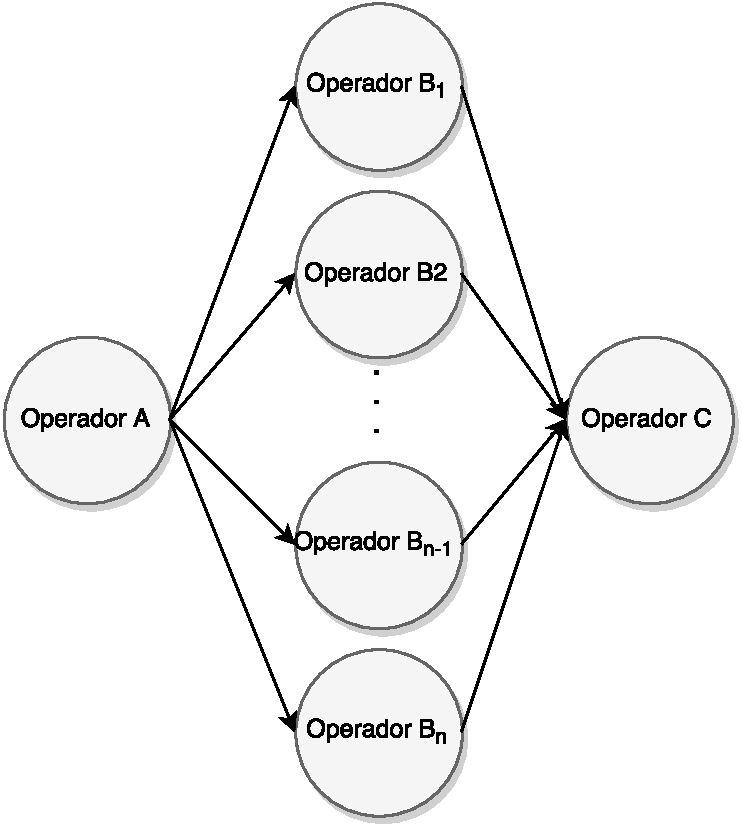
\includegraphics[scale=0.55]{images/Elasticidad.pdf}
	\caption{Elasticidad en un SPS.}
	\label{fig:elasticidad}
\end{figure}

Un ejemplo pr\'actico de elasticidad es el supermercado, donde se debe considerar la cantidad de cajas necesarias para atender de manera eficiente los clientes que van llegando en un per\'iodo de tiempo. Si se estudia el per\'iodo de la ma\~nana, en general, se tiene un bajo flujo de personas que acude al supermercado, en comparaci\'on con la tarde, pero alto comparado la medianoche. Por lo tanto, en los horarios de la tarde es necesario poseer una mayor cantidad de cajas disponibles que en la ma\~nana, disminuyendo la cantidad nuevamente cuando el horario bordea la medianoche, adapt\'andose, de forma el\'astica, la cantidad de cajas disponibles en el supermercado al flujo de gente.

En el trabajo realizado, se propone un sistema el\'astico basado en la carga de los operadores. De esta manera, seg\'un el tr\'afico recibido se aumentan o disminuyen el n\'umero de los operadores, de tal manera de mantener \normalsize{un rendimiento eficiente} en el tiempo, disminuyendo el riesgo de sobrecarga y con ello la p\'erdida de datos.

\section{MAPE}
\label{sec:MAPE}
\normalsize{MAPE (Monitor-Analyze-Plan-Execute) es un modelo basado en m\'odulos, cuyo objetivo es la adaptabilidad del sistema seg\'un condiciones externas} \citep{ibm2005architectural}. \normalsize{Para el manejo autom\'atico de los recursos del sistema, se propone implementar un control inteligente bajo ciclos.}

\normalsize{En la Figura} \ref{fig:mape} \normalsize{se muestra una arquitectura dise\~nada bajo cuatro m\'odulos para la administraci\'on autom\'atica del sistema:}

\begin{itemize}
	\item \normalsize{Monitor: Este m\'odulo provee los mecanismo de recolecci\'on, a\~nadiendo filtros o alg\'un operador necesario para la administraci\'on de los recursos.}
	\item \normalsize{An\'alisis: Este m\'odulo utiliza modelos matem\'aticos, ya sea series de tiempo o modelos de colas, para el an\'alisis de la informaci\'on entrante. Con esto mismo, se espera realizar un aprendizaje del sistema, para posteriormente ayudar en la predicciones futuras por parte del modelo matem\'atico.}
	\item \normalsize{Planificaci\'on: Este m\'odulo designa las acciones necesarias para cumplir con los objetivos y las metas necesarias del sistema. En general, se dise\~nan pol\'iticas para la planificaci\'on de las tareas.}
	\item \normalsize{Ejecuci\'on: Este m\'odulo est\'a encargado en ejecutar la planificaci\'on elaborada seg\'un las necesidades din\'amicas del sistema.}
\end{itemize}

\begin{figure}[!ht]
	\centering
	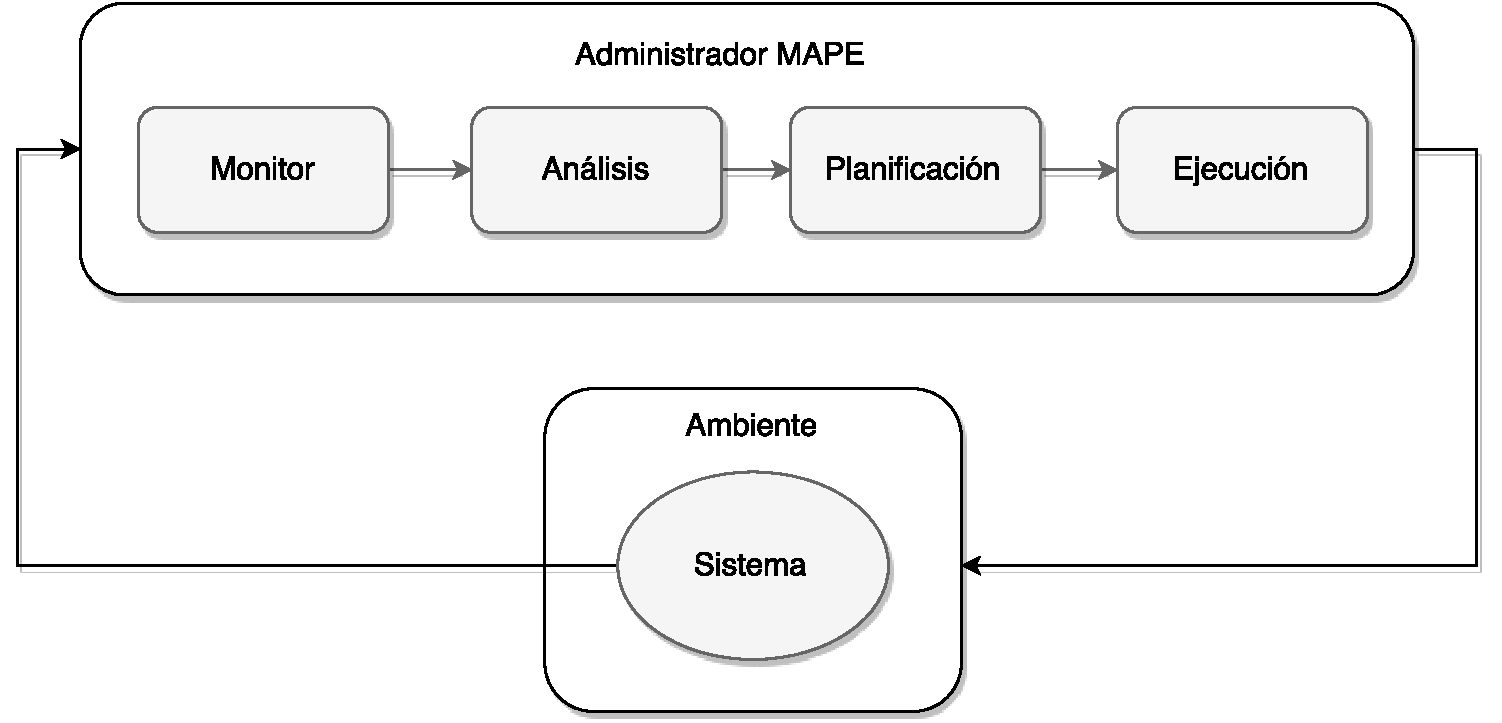
\includegraphics[scale=0.55]{images/MAPE.pdf}
	\caption{Ejemplo de un sistema con un administrador basado en MAPE.}
	\label{fig:mape}
\end{figure}

\section{Procesos estoc\'asticos}
\label{sec:procesosEstocasticos}

Se define un proceso estoc\'astico como una colecci\'on de variables aleatorias {$X_t$, con $t ~ \epsilon ~ T$}, las cuales est\'an determinadas por alg\'un comportamiento en el tiempo $t$. Esto significa que cada variable se comporta de cierta manera en el tiempo, sin poseer un proceso determin\'istico entre sus variables, es decir, que las variables dependan de la historia \citep{taylor2014introduction}.

Esto permite definir un estado como el posible comportamiento que puede tener una variable aleatoria en el sistema. Para ejemplificar, considera un modelo que contemple tres estados: estable, inestable y ocioso, y seg\'un el valor de la variable aleatoria, vaya cambiando de un estado a otro. Un caso de estudio utilizando el concepto de estados son las cadenas de Markov, las cuales consideran distintos estados, donde cada uno representa un comportamiento del sistema \citep{de1978calculus}.

Las cadenas de Markov son procesos estoc\'asticos, las cuales han sido utilizadas para permitir la predicci\'on de carga en modelos como el propuesto por \citep{GongGW10}. En este trabajo se definen estados que son independientes en el transcurso del tiempo, con el fin de realizar an\'alisis a futuro tomando en consideraci\'on los datos \textit{a priori}.

\subsection{Cadena de Markov}
\label{subsec:cadenaMarkov}

Sea $X_t$ el valor de una variable aleatoria $X$ en un tiempo $t$, donde el conjunto de todos los valores posibles para $X$ se denominada espacio de estado \citep{ching2006markov}. La variable aleatoria es un proceso de Markov, si s\'olo y si las probabilidades de transici\'on entre dos estados de $\Omega$ (definido como el universo de posibles estados), s\'olo depende del estado actual, como se denota en la Ecuaci\'on \ref{eq:defMarkov} y gr\'aficamente en la Figura \ref{fig:procesoMarkov}. Cabe destacar que este tipo de proceso es un caso espec\'ifico de los procesos estoc\'asticos.

\begin{equation} \label{eq:defMarkov} 
	P_r(X_{t+r} = S_j | X_0 = S_k ; X_1 = S_l ; ... ; X_t = S_i) = P_r(X_{t+1} = S_j | X_t = S_i)
\end{equation}

\begin{figure}[ht!]
  \centering
    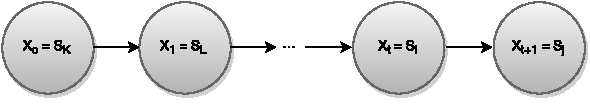
\includegraphics[scale=0.6]{images/ProcesoMarkov.pdf}
  \caption{Proceso de Markov.}
  \label{fig:procesoMarkov}
\end{figure}

Una cadena de Markov es una secuencia de variables aleatorias generadas por un proceso de Markov, como se denota en la Ecuaci\'on \ref{eq:cadenaMarkov}.

\begin{equation} \label{eq:cadenaMarkov}
	(X_0, X_1, X_2, ..., X_{n-1}, X_{n})
\end{equation}

\normalsize{Donde en la Ecuaci\'on} \ref{eq:transicionMarkov} \normalsize{se define la cadena bajo las probabilidades de transici\'on existentes en \'este.} En la Figura \ref{fig:cadenaMarkov} se muestra un ejemplo de la transici\'on del estado $i$ al estado $j$, dada la probabilidad $P_{ij}$.

\begin{equation} \label{eq:transicionMarkov}
	P_{ij} = P_r(i \rightarrow j) = P_r(X_{t+1} = S_j | X_t = S_i)
\end{equation}

\begin{figure}[ht!]
  \centering
    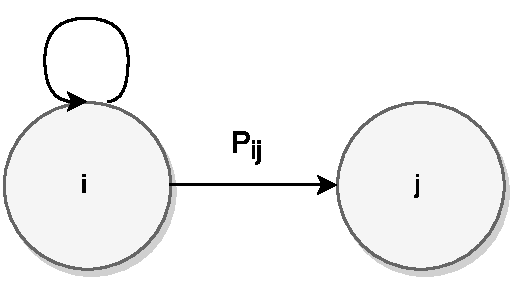
\includegraphics[scale=0.6]{images/CadenaMarkov.pdf}
  \caption{Cadena de Markov.}
  \label{fig:cadenaMarkov}
\end{figure}

En la Ecuaci\'on \ref{eq:matrizTransicion} se presenta una matriz de transici\'on de estados finitos, \normalsize{donde} $P_ij$ \normalsize{la probabilidad de pasar de un estado a otro. Las probabilidades son tales que la suma de todas las transiciones de un estado a otro debe ser igual a 1.}

\begin{equation} \label{eq:matrizTransicion}
	P =
	\begin{bmatrix}
		P_{1,1} & P_{1,2} & \cdots & P_{1,n} \\
		P_{2,1} & P_{2,2} & \cdots & P_{2,n} \\
		\vdots  & \vdots  & \ddots & \vdots  \\
		P_{n,1} & P_{n,2} & \cdots & P_{n,n} \\
	\end{bmatrix}
	\hspace*{1cm} \sum_{j=1}^{n} P_{ij} = 1 ; \forall i
\end{equation}

En la Figura \ref{fig:ejCadenaMarkov} se muestra un ejemplo de una cadena de Markov simple, donde se analiza la probabilidad del clima de ma\~nana dado el clima de hoy d\'ia. Como se puede observar, no se considera la historia del clima en la semana, s\'olo el del caso actual, tal como es definido en los procesos estoc\'asticos. Las probabilidades \normalsize{de transici\'on} de un clima a otro, se pueden ver en la Ecuaci\'on \ref{eq:ejCadenaMarkov}.

\begin{figure}[ht!]
	\centering
	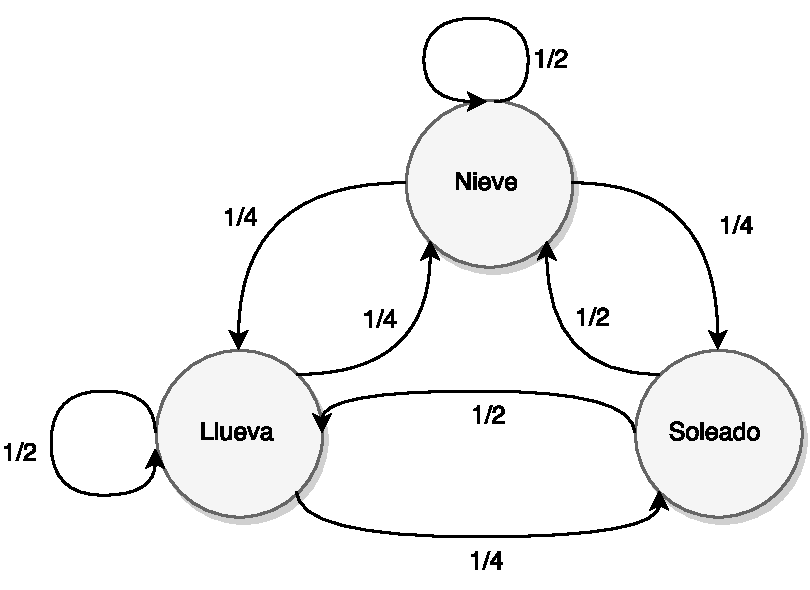
\includegraphics[scale=0.5]{images/EjCadenaMarkov.pdf}
	\caption{Ejemplo de cadena de Markov.}
	\label{fig:ejCadenaMarkov}
\end{figure}

\begin{equation} \label{eq:ejCadenaMarkov}
	P =
	\begin{bmatrix}
		\frac{1}{2} & \frac{1}{4} & \frac{1}{4} \\
		\frac{1}{2} & 0 & \frac{1}{2} \\
		\frac{1}{4} & \frac{1}{4} & \frac{1}{2}
	\end{bmatrix}	
\end{equation}

\normalsize{Dentro de las cadenas de Markov existen clasificaciones, las cuales son requisitos para realizar c\'alculos como la distribuci\'on estacionaria. Una de ellas son las cadenas irreductibles, esto significa que todos sus estados son accesibles entre ellos, por lo tanto existe una posible transici\'on de un estado a otro, habiendo una \'unica clase de estados, por lo tanto, todo estado debe cumplir con la Ecuaci\'on} \ref{eq:accesibleMarkov}. \normalsize{En la Figura} \ref{fig:ejCadenaMarkov-Reductible} \normalsize{se presenta un ejemplo de cadena reductible, donde no existe trancaron posible luego de llegar al estado \textit{Lluvia}. A diferencia de la cadena de la Figura} \ref{fig:ejCadenaMarkov}, \normalsize{donde todos los estados pueden realizar una transici\'on a otro estado.}

\begin{equation} \label{eq:accesibleMarkov}
	P_{ij}^{(n)} = P(X_n = j | X_0 = i) > 0
\end{equation}

\begin{figure}[ht!]
	\centering
	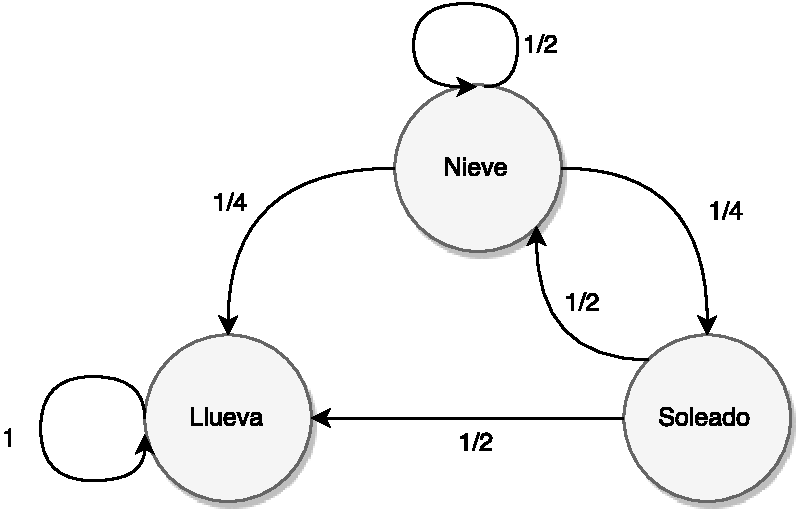
\includegraphics[scale=0.5]{images/EjCadenaMarkov-Reductible.pdf}
	\caption{Ejemplo de cadena de Markov reductible.}
	\label{fig:ejCadenaMarkov-Reductible}
\end{figure}

\normalsize{Una de las definiciones atribuidas a un estado es la periodicidad, esto significa que es la cantidad de transiciones necesarias para volver al mismo estado desde donde se inicio la transici\'on original, definida por el valor $d$. En la Ecuaci\'on} \ref{eq:periodicidadMarkov} \normalsize{indica la condici\'on para cumplir con la periodicidad, donde $d$ es el mayor valor posible de $n$, siendo este \'ultimo el \'indice de la transici\'on realizada. En el caso que la cantidad de transiciones sea mayor a 1 significa que el estado es peri\'odico, y en el caso que sea 1 se denomina aperi\'odico. En la Figura} \ref{fig:ejCadenaMarkov} \normalsize{se presenta una cadena con dos estados aperi\'odicos y uno peri\'odico, debido que el estado \textit{Soleado} posee $d=2$, dado que para volver a si mismo debe realizar dos transiciones en la cadena.}

\begin{equation} \label{eq:periodicidadMarkov}
	P_{ii}^{(n)} = P(X_n = i | X_0 = i) > 0 ; n = {d,2d,3d,..., m \cdot d}
\end{equation}

\begin{figure}[ht!]
	\centering
	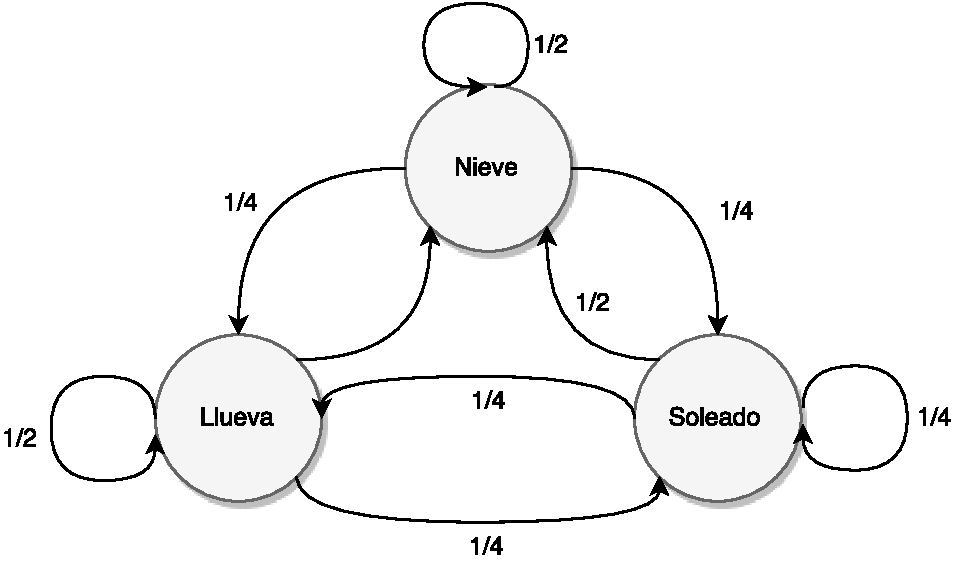
\includegraphics[scale=0.5]{images/EjCadenaMarkov-Aperiodica.pdf}
	\caption{Ejemplo de cadena de Markov con estados aperi\'odicos.}
	\label{fig:ejCadenaMarkov-Aperiodica}
\end{figure}

\normalsize{Sea $F(i,i)$ la probabilidad que se posee que despu\'es de $k$ transiciones se retorne al estado $i$, el cual se define seg\'un la Ecuaci\'on} \ref{eq:recurrentedMarkov}. \normalsize{En el caso que $F(i,i)=1$ se define este estado como recurrente, y en caso contrario, es transitorio. En el caso que se posea una cadena con un n\'umero finito de estados y \'este sea recurrente, entonces \'este es recurrente positivo. De haber un n\'umero infinito de estados, entonces el estado es recurrente nulo.}

\begin{equation} \label{eq:recurrentedMarkov}
	F(i,i) = \sum_{k=1}^{\infty}{F_k(i,i)}
\end{equation}

Por otra parte, la probabilidad que la cadena est\'e en el estado $S_i$ en el tiempo $t+1$, est\'a dada por la ecuaci\'on de Chapman-Kolmog\'orov \citep{Papoulis1984}, la cual se muestra en la Ecuaci\'on \ref{eq:chapman-kolmogorov1}.

\begin{equation} \label{eq:chapman-kolmogorov1}
\begin{split}
	\Pi_{i} (t+1) &= P_r(X_{t+i}=S_i) \\
				  &= \sum _{k} P_r(X_{t+i} = S_i / X_t = S_k) \cdot P_r(X_t = S_k)\\
				  &= \sum _{k} P_r(X_{t+i} = S_i / X_t = S_k) \cdot \Pi_{k} (t)
\end{split}	
\end{equation}

Y en notaci\'on matricial en la Ecuaci\'on \ref{eq:chapman-kolgorov2}.

\begin{equation} \label{eq:chapman-kolgorov2}
\begin{split}
	\Pi_{(t+1)} &= \Pi_{(t)}P\\
	\begin{bmatrix}
		\Pi_1 & \Pi_2 & \Pi_3
	\end{bmatrix} _{(t+1)}
	&= \begin{bmatrix}
		\Pi_1 & \Pi_2 & \Pi_3
	\end{bmatrix} _{(t)}
	\begin{bmatrix}
		P_{1,1} & P_{1,2} & \cdots & P_{1,n} \\
		P_{2,1} & P_{2,2} & \cdots & P_{2,n} \\
		\vdots  & \vdots  & \ddots & \vdots  \\
		P_{n,1} & P_{n,2} & \cdots & P_{n,n}
	\end{bmatrix}
\end{split}
\end{equation}

\normalsize{En caso que la cadena sea irreducible y sus estados sean recurrentes positivos aperi\'odicos}, entonces se puede calcular la distribuci\'on estacionaria como se muestra la Ecuaci\'on \ref{eq:chapman-kolgorov3}, la cual indica el comportamiento a futuro de la cadena de Markov, dado los estados y transiciones que \'este posee.

\begin{equation} \label{eq:chapman-kolgorov3}
\begin{split}
	\Pi (t) &= \Pi (t-1)P \\
				  &= \Pi (t-2)P^{2}\\
				  &= \Pi (0)P^{t}\\
\end{split}
\end{equation}

\normalsize{Donde $\Pi (0)$ es la distribuci\'on inicial de la cadena.}

\subsection{Trabajo relacionado}
\label{subSec:markovTrabajo}
Existen modelos predictivos \normalsize{que} simulan el comportamiento del sistema, ya sea del flujo o de la carga de un operador, de tal manera que pueden predecir cual es su estado en un tiempo futuro. En general, para poder realizar una predicci\'on se analizan las variables en una ventana de tiempo, para posteriormente aplicar un modelo matem\'atico que prediga la variaci\'on del sistema en la pr\'oxima ventana de tiempo que se tiene estipulada.

Dentro de las aplicaciones que se han realizado con modelos predictivos, se encuentra PRESS \citep{GongGW10}. Este sistema orientado a \textit{Cloud Computing}, analiza la cantidad de recursos disponibles, ya sea la memoria disponible o el uso promedio de CPU en las m\'aquinas virtuales que se disponen en el \textit{Cloud}. Para realizar la predicci\'on del estado del sistema, se aplica un modelo basado en cadenas de Markov, tomando sus estados como ventanas de tiempo en un determinado per\'iodo. De esta manera, se analiza el estado del sistema en un tiempo en espec\'ifico para ver si posee correlaci\'on con alg\'un estado de la cadena de Markov, para ver la transici\'on de ese estado a otro y construir la matriz de transici\'on. Posteriormente, con la ecuaci\'on de Chapman-Kolmogorov, se calcula la distribuci\'on estacionaria de la matriz de transici\'on, de tal manera de saber en \normalsize{qu\'e} estado est\'a en la pr\'oxima ventana de tiempos para finalmente analizar si es necesario alg\'un cambio en el sistema.

Dentro de la misma l\'inea de modelos predictivos existe el sistema AGILE \citep{NguyenSGSW13} para \textit{Cloud Computing} que modifica el n\'umero de m\'aquinas virtuales de forma din\'amica en un \textit{Cloud}. Este trabajo aplica la transformada de Fourier \citep{falk2012first} a series temporales obtenidas mediante el muestreo de la carga de CPU en una ventana de tiempo. Luego, la funci\'on resultante se analiza con distintas frecuencias, de tal manera de determinar la predicci\'on de la pr\'oxima ventana de tiempo a cada una de las funciones creadas. De esta manera, se sintetizan \normalsize{todas las predicciones} realizadas por cada funci\'on para analizar el comportamiento del sistema en la pr\'oxima ventana de tiempo, y ver si es necesario aumentar o disminuir recursos de \'este.

\section{Teor\'ia de colas}
\label{sec:teoriaColas}

La teor\'ia de colas se centra en el estudio matem\'atico de las colas existentes en un sistema, cuyo caso de estudio \normalsize{es el \textit{performance} del servidor seg\'un el n\'umero de clientes que se posea} \citep{cooper1972introduction}. En la Figura \ref{fig:teoriaColas} se muestra un ejemplo de un sistema basado en teor\'ia de colas, donde existen $n$ productores que env\'ian tareas a $m$ servidores disponibles, y en caso de no estar disponibles se genera una cola de espera en el sistema. Los elementos del sistema son:

\begin{itemize}
	\item \textbf{Productor}: es qui\'en provee la fuente de datos de entrada para el servidor.
	\item \textbf{Cola o l\'inea de espera}: la cual est\'a encargada de almacenar provisionalmente la informaci\'on emanada por el productor en caso que los servidores est\'en ocupados, para que posteriormente sean procesados.
	\item \textbf{Servidor}: es qui\'en procesa la informaci\'on disponible en la cola, de tal manera de entregar una fuente de salida con la informaci\'on procesada.
\end{itemize}

\begin{figure}[!ht]
	\centering
	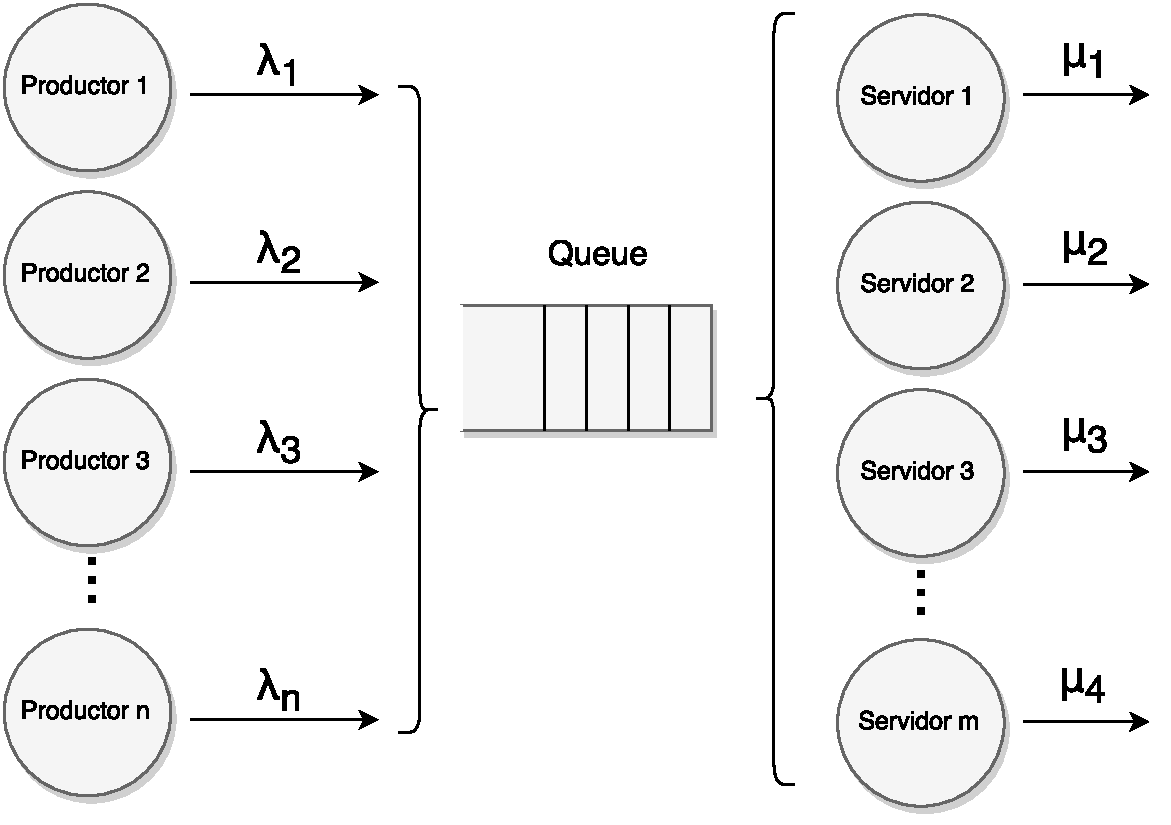
\includegraphics[scale=0.6]{images/TeoriaColas.pdf}
	\caption{Ejemplo de un sistema basado en teor\'ia de colas.}
	\label{fig:teoriaColas}
\end{figure}

Otros componentes importantes en el sistema, son definidos a continuaci\'on:
\begin{itemize}
	\item \textbf{Tasa de llegada}: denotado $\lambda$, es la cantidad de datos, eventos o informaci\'on que van llegando en un determinado per\'iodo de tiempo, la cual est\'a determinada por los productores que existen en el sistema.
	\item \textbf{Tasa de procesamiento}: denotado $\mu$, tambi\'en llamada tasa de servicio, es la cantidad de datos, eventos o informaci\'on que salen del sistema, producto del procesamiento provisto por cada servidor.
	\item \textbf{Tasa de rendimiento}: denotado $\rho$, es el porcentaje de utilizaci\'on del sistema, definido como $\rho = \frac{\lambda}{s\mu}$, siendo $s$ la cantidad de servicios disponibles, definiendo as\'i un sistema estable si es que $\rho < 1$, dado que la capacidad de procesamiento es mayor que la tasa de llegada.
	\item \textbf{Disciplina de la cola}: Pol\'itica utilizada para extraer los datos encolados en el sistema. Alguna de las pol\'iticas tradicionales son: \textit{FIFO}, \textit{LIFO}, \textit{RSS}, entre otros.
\end{itemize}

Este tipo de modelo se puede aplicar a los SPS de manera directa, debido a que el operador emisor o la fuente de datos es el productor, y el operador receptor es el servidor del sistema. Sin embargo existe un problema interesante a analizar asociado a las a la carga de los operadores. Por ejemplo, si se tiene un operador con una tasa de llegada $\lambda$ y una tasa de servicio $\mu$, donde $\mu < \lambda$, se tiene un sistema inestable, debido que se procesa m\'as lento de lo que llegan los datos. Esto genera colas por lo que es necesario un aumento del rendimiento del sistema, por lo que es necesario modificar la cantidad de operadores.